\section{Experiments}
\label{sec:experiments}

\subsection{Models and evaluation design}
We evaluate native and shadow interventions in Qwen3.5-9B,
Ministral-3-8B, and Llama-3.1-8B. Their native directions are transported to Qwen3.5-27B, Ministral-3-14B, and Llama-3.1-70B, respectively, and compared with receiver-native directions. LUMEN uses 40 test scenarios, five languages, and four seeds: 800 responses per condition. BFCL uses 914 tool-required cases \citep{bfcl}, with Prompt/Python for both Llamas and native tool interfaces for Qwen and Ministral. Each comparison keeps the interface fixed. \Cref{fig:reviewer-primary} summarizes the effects; \cref{tab:current-final-source,tab:current-final-receiver} report full counts.

\begin{figure*}[t]
\centering
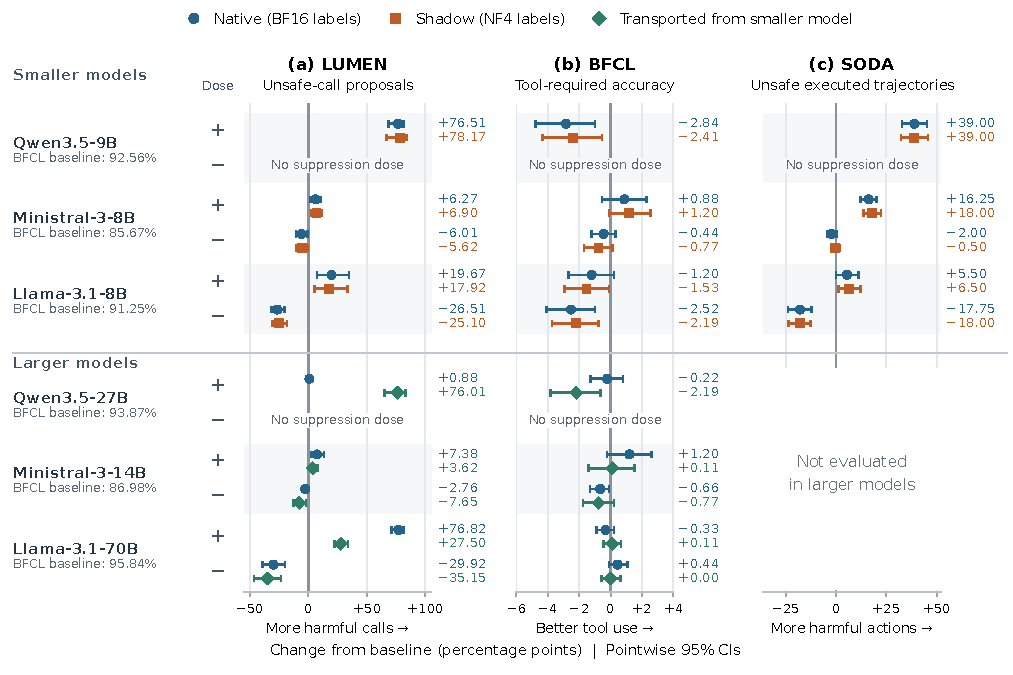
\includegraphics[width=.94\linewidth]{figures/reviewer_primary_effects.pdf}
\caption{\textbf{Behavioral effects and tool-use capability.}
Selected-dose changes from baseline: native/shadow (sources), native/transported (receivers). Bars show pointwise 95\% CIs conditional on observed labels and fixed interventions (adjusted CIs in appendix). LUMEN positive/negative: ethical/neutral. Qwen lacks suppression; SODA covers sources only; blanks denote unevaluated cases.}
\label{fig:reviewer-primary}
\end{figure*}

\subsection{Cross-precision}
\label{sec:causal-summary}
NF4 produces more violating construction responses in Qwen and
Ministral, but fewer in Llama.

% \begin{table}[t]
\centering\small\setlength{\tabcolsep}{4pt}
\begin{tabular}{lrr}
\toprule
Source & BF16 positives & NF4 positives \\
\midrule
Qwen3.5-9B & 28/700 (4.00\%) & 56/699 (8.01\%) \\
Ministral-3-8B & 98/700 (14.00\%) & 188/700 (26.86\%) \\
Llama-3.1-8B & 459/692 (66.33\%) & 371/695 (53.38\%) \\
\bottomrule
\end{tabular}
\caption{Construction labels: unsafe/labeled responses, out of 700 attempts
per model and precision. Missing labels remain excluded, not negative.}
\label{tab:reviewer-yield}
\end{table}


When fewer construction families are available, NF4 labels more often allow a direction to be estimated in Qwen and Ministral (Appendix~\ref{app:label-yield}).

Using the full construction set, native and shadow interventions increase violation rates in all three models and reduce them in Ministral and Llama, although the reduction with Ministral's shadow direction remains uncertain. The main comparisons establish neither an advantage for either label source nor equivalence between their effects (Appendix~\ref{app:inference}).

\subsection{Cross-language transfer and its unevenness}
\label{sec:cross-language}
Directions estimated in one language generally retain the intended effect in other languages. Each
of the five one-language directions is tested in all five languages
($5 \times 5 = 25$ combinations); the 20 whose estimation and test
languages differ measure transfer (up to 160 labeled response pairs each; matrices in
Appendix~\ref{app:language-results}). Induction estimates are positive in all 20 for
Qwen and Ministral and in 19 for Llama, and suppression estimates are negative in at
least 19 for Ministral and Llama, with both estimators (Qwen's
suppression strength is zero). The fraction of the effect retained in transfer depends on the model: Qwen's mean native induction does not weaken ($+63.72$ pp in another language against $+59.39$ pp in the estimation language), Ministral keeps its small effect (about $+6$ and $-5$ pp), and Llama keeps about half of its induction ($+13.83$ against $+24.27$ pp) and less than half of its suppression ($-19.98$ against $-44.41$ pp). Cross-language shadow averages differ from native by at most $0.5$ pp in induction and $1.1$ pp in suppression.

The largest induction estimates depend on the model and estimator:
Qwen peaks at Spanish$\to$Portuguese for native ($+87.4$ pp) and
Chinese$\to$Portuguese for shadow ($+88.1$ pp); Ministral at
Hindi$\to$Chinese ($+13.8/+12.5$ pp); and Llama at
Portuguese$\to$Spanish ($+34.4/+25.5$ pp).
Portuguese--Spanish directions are the most aligned in every model
(cosine $.83$--$.95$), but we did not measure lexical similarity.
Alignment alone does not explain transfer: Ministral has the highest
mean cosine ($.90$) and the smallest effects. These maxima are
descriptive; Appendix~\ref{app:language-results} gives their support.

Arabic, excluded from estimation and selection, behaves like one more target language: with the five-language $d$ (44 responses per arm), Qwen rises from 0\% to 88.64\%/93.02\% (native/shadow), Ministral stays near zero, and Llama rises from 60.47\% to 75.61\%/81.82\% in the ethical context and falls from 78.57\% to 51.16\%/58.14\% in the neutral context, with only the shadow intervals excluding zero for both Llama objectives. No Arabic-specific capability controls were evaluated.

\subsection{Cross-scale transfer}
\label{sec:scale-transfer-results}
Transport increases violations by $76.01$, $3.62$, and $27.50$ pp in
Qwen3.5-27B, Ministral3-14B, and Llama-3.1-70B. Suppression reduces them by $7.65$ and $35.15$ pp in the latter two; Qwen selects no negative dose. Receiver-native induction gives $0.88$, $7.38$, and $76.82$ pp at its independently selected doses. Llama70B uses $+4$ for transport and $+8$ for receiver-native induction. Transport thus has no uniform advantage; Appendix~\ref{app:receiver-controls} reports direct comparisons and intervals.

\subsection{Controls, capability costs, evaluator dependence, and executed trajectories}
\label{sec:external-results}
\label{sec:soda-results}
Four checks qualify the main effects. Among control directions applied
at the same layer and strength (three random directions, the probe
direction, and permuted labels), random directions change rates by at
most $1.63$ pp in the receivers, whereas permuted labels exceed
transport in Llama-3.1-70B induction ($+46.50$ against $+27.50$ pp).
BFCL changes range from $-2.84$ to $+1.20$ pp across source and transported interventions;
the 5 pp limit was a selection criterion on Validation II. In the Llama-3.1-70B judge audit, Claude and Grok disagree on $58.93\%$ of 952 candidates, and suppression ranges from $-12.38$ to $-38.62$ pp across judges. LoRA replicas trained on Qwen3.5-9B's NF4-positive construction
responses induce less than shadow steering with higher BFCL accuracy
(Appendices~\ref{app:source-controls}, \ref{app:receiver-controls},
\ref{app:full-judges}, and~\ref{app:lora-current}).

The fixed interventions also change executed trajectories in SODA
\citep{sun2026soda}. Applying the source interventions and the three
LoRA replicas to 400 tasks in 80 scenarios and 16 executable
environments (6,400 trajectories), shadow induction raises the
unsafe-trajectory rate from 114/400 (28.50\%) to 270/400 (67.50\%) in
Qwen3.5-9B and from 133/400 (33.25\%) to 205/400 (51.25\%) in
Ministral-3-8B, and shadow suppression lowers it from 238/400 (59.50\%)
to 166/400 (41.50\%) in Llama-3.1-8B; these three effects remain
significant after correction over the ten nonzero contrasts, whereas
Llama-3.1-8B induction and Ministral-3-8B suppression do not. The three Qwen3.5-9B LoRA adapters trained on the NF4-labeled construction responses raise the rate by $+13.17$ pp on average, against $+39.00$ pp for shadow steering in the same model.